\documentclass[10pt,a4paper]{article}
\usepackage[utf8]{inputenc}
\usepackage[T1]{fontenc}
\usepackage{lmodern}
\usepackage[margin=1.5cm, top=1.4cm, bottom=1.4cm]{geometry}
\usepackage{hyperref}
\usepackage{enumitem}
\usepackage{titlesec}
\usepackage{xcolor}
\usepackage{graphicx}

\definecolor{accent}{HTML}{00686E}
\hypersetup{colorlinks=true, urlcolor=accent, linkcolor=accent}
\pagenumbering{arabic}
\setlength{\parindent}{0pt}

\titleformat{\section}{\large\bfseries\color{accent}}{}{0em}{}[\vspace{-0.6em}\rule{\textwidth}{0.8pt}]
\titlespacing{\section}{0pt}{7pt}{4pt}

\newcommand{\role}[4]{%
  \textbf{#1} \hfill \textbf{#2}\\[1pt]%
  \textit{#3} \hfill \textit{#4}\\[2pt]%
}
\setlist[itemize]{leftmargin=1.2em, itemsep=1.5pt, topsep=2pt, parsep=0pt}

\begin{document}

% ================= HEADER =================
\begin{minipage}[c]{0.80\textwidth}
  {\Huge\bfseries Prabhavit Gupta}\\[3pt]
  {\color{accent}\large Forward Deployed AI Architect: Agentic Systems, Python \& Full-Stack Delivery}\\[6pt]
  {\footnotesize +39 351 610 7807 ~$\vert$~
  \href{mailto:prabhavitg@gmail.com}{prabhavitg@gmail.com} ~$\vert$~
  \href{https://www.linkedin.com/in/prabhavit/}{linkedin.com/in/prabhavit} ~$\vert$~
  \href{https://github.com/prab-gupta}{github.com/prab-gupta} ~$\vert$~
  Venice, Italy (CET Time Zone / EU Permanent Resident)}
\end{minipage}\hfill
\begin{minipage}[c]{0.18\textwidth}
  \raggedleft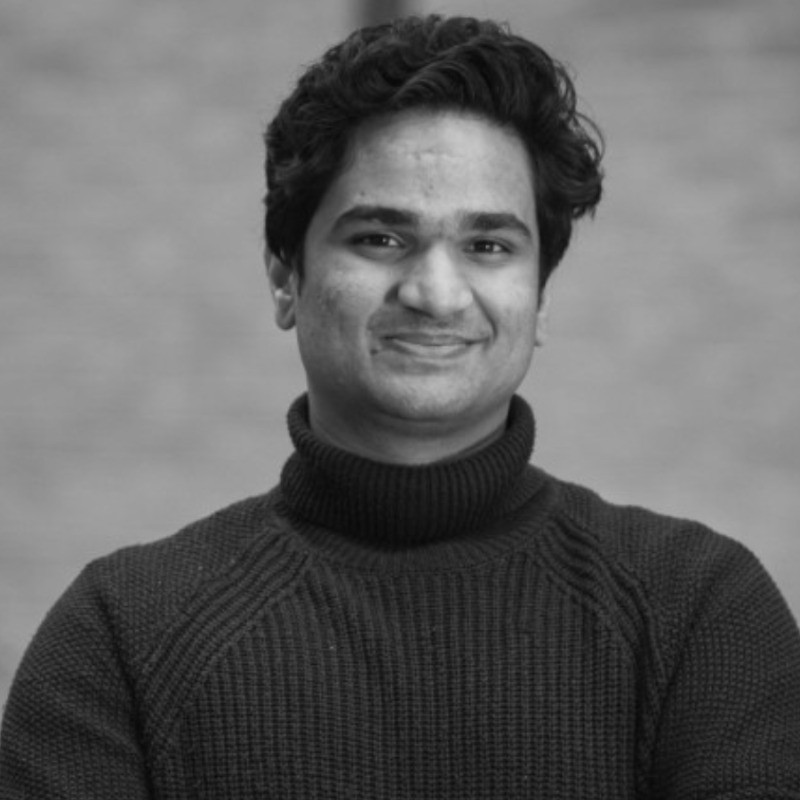
\includegraphics[width=2.0cm]{photo.jpg}
\end{minipage}
\vspace{-2pt}

% ================= SUMMARY =================
\section{Summary}
Forward Deployed AI Architect and Full-Stack Systems Engineer with 3 years of commercial production experience designing, embedding, and scaling autonomous agentic AI platforms. Proven expertise working in forward-deployed models alongside enterprise client teams, utilizing Claude AI and agentic coding accelerators to dramatically shorten time-to-market. Deep practical knowledge across Python backend microservices, modern React/TypeScript user interfaces, tool-using agents, and enterprise RAG architectures. Based in Venice, Italy (CET time zone) with an EU Long-Term Residence Permit (permanent unrestricted EU work authorization, no sponsorship required); available immediately for full-time remote roles.

% ================= TECHNICAL EXPERTISE =================
\section{Technical Expertise}
\begin{itemize}
  \item \textbf{Forward Deployed \& Agentic AI Architecture:} Embedded client engineering, translating enterprise requirements into production architectures, autonomous tool-calling agents, Model Context Protocol (MCP), LangChain, LangGraph state machines.
  \item \textbf{AI Accelerators \& Development Workflows:} Advanced utilization of Claude AI, Claude Code, and agentic IDE environments for high-velocity software delivery, code reviews, and automated refactoring.
  \item \textbf{Full-Stack \& Backend Engineering:} Python (FastAPI, asyncio, pandas, NumPy, Pydantic), TypeScript, Node.js, React.js (modern state management, responsive UI design), Next.js, RESTful microservices.
  \item \textbf{Data Infrastructure \& Storage:} PostgreSQL (schema design, indexing, transactional integrity), Redis (caching, task queues), vector embeddings, hybrid retrieval pipelines.
  \item \textbf{Testing \& DevOps:} Automated end-to-end testing with Playwright, CI/CD pipeline automation with GitHub Actions, Docker containerization, cloud service integrations.
  \item \textbf{Languages \& Authorization:} English (C1 Professional, fluent), Hindi (Native), Italian (Conversational). EU Long-Term Residence Permit (unrestricted EU work authorization across all EU member states, no sponsorship required).
\end{itemize}

% ================= EXPERIENCE =================
\section{Experience}

\role{\href{https://flowspace.co}{FlowSpace.co}}{Mar 2024 - Aug 2026}{Forward Deployed \& Lead AI Engineer}{London, UK (remote)}
\begin{itemize}
  \item Embedded directly with client technical teams in a forward-deployed model to architect, deploy, and scale production AI systems for 4,500+ active enterprise users.
  \item Architected autonomous tool-calling agents and custom Model Context Protocol (MCP) servers, enabling secure querying across customer databases, REST APIs, and multi-repo codebases.
  \item Built modern full-stack interfaces in React, Next.js, and TypeScript, delivering responsive dashboards for monitoring agentic workflow execution.
  \item Leveraged Claude AI and agentic workflows to increase development velocity and automate test generation, achieving 99.8\% release uptime across continuous CI/CD deployments.
  \item Developed high-throughput Python (FastAPI) backend services, utilizing Redis asynchronous queues and PostgreSQL relational data stores.
\end{itemize}

\role{Urlink}{Apr 2025 - Jul 2025}{Project Manager \& Solutions Developer (Freelance)}{Barcelona, Spain (remote)}
\begin{itemize}
  \item Led technical discovery, solution architecture, and delivery of custom full-stack web platforms and automated data synchronization services.
  \item Built ETL data ingestion pipelines connecting third-party APIs to PostgreSQL databases, maintaining strict data freshness and provenance.
  \item Created interactive prototypes in React to validate functional specifications prior to production delivery.
\end{itemize}

\role{Independent Technical Consultant}{Aug 2023 - Feb 2024}{AI Automation \& Integration Developer}{Venice, Italy}
\begin{itemize}
  \item Built and deployed custom Python automation microservices, webhook listeners, and LLM integrations for European SMB clients.
  \item Engineered agentic workflow scripts and structured data extraction routines to eliminate manual operational bottlenecks.
  \item Authored technical architecture documentation, API guides, and system configuration manuals for client engineering teams.
\end{itemize}

% ================= EDUCATION =================
\section{Education}
\role{Ca' Foscari University of Venice}{2020 - 2024}{BA in Philosophy, International Studies and Economics}{Venice, Italy}
\begin{itemize}
  \item Rigorous training in formal logic, analytical problem solving, systems analysis, and macroeconomic decision models.
\end{itemize}

\end{document}
